\documentclass{beamer} % Création d'un document beamer
\usepackage[utf8]{inputenc} %utf = l'option de inputenc/le type d'encodage (Ecriture fr), inputenc permet de mettre les caractères spéciaux (par ex les accents)
\usepackage[T1]{fontenc} % fontenc permet de prendre correctement ces caractères spéciaux dans le fichier de sortie, T1 est le type d'encodage
\usetheme{Warsaw} % Dîtes moi le thème que vous voulez : (http://mcclinews.free.fr/latex/beamergalerie/completsgalerie.html)  Warsaw est bien sinon Ilmenau.
\setbeamercolor{normal text}{fg=black} % Couleur du texte basique
\setbeamercolor{frametitle}{fg=white} % Couleur des titres des frames
\graphicspath{{Images/}} % Le chemin pour les images, cela nous évite de devoir écrire Images/nom image en écrivant seulement image
%\usefontheme{structureitalicserif} %Choix de la police 
\usepackage{xcolor}%Permet d'utiliser des couleurs
%\usepackage{enumitem}%Permet de modifier les itemize // !!!créé des conflits avec beamer!!!
%\usepackage{tikz}%Pour les figures
%Il est possible de changer les blocks (leur couleur ou de les mettre en colonne par exemple. (http://mcclinews.free.fr/latex/introbeamer/elements_contenu.html) (http://deic.uab.es/~iblanes/beamer_gallery/individual/CambridgeUS-default-professionalfonts.html)
%\includegraphics[Height= cm, width= cm, scale= cm]{fichier source} Pour les include graphics

\title{Optimisateur de WarGame}
\author{Elie MALBEC - Alex LEFEVRE - Yoann Kablan \\
\small{{ 21805304 - 21809848 - }}}
\date{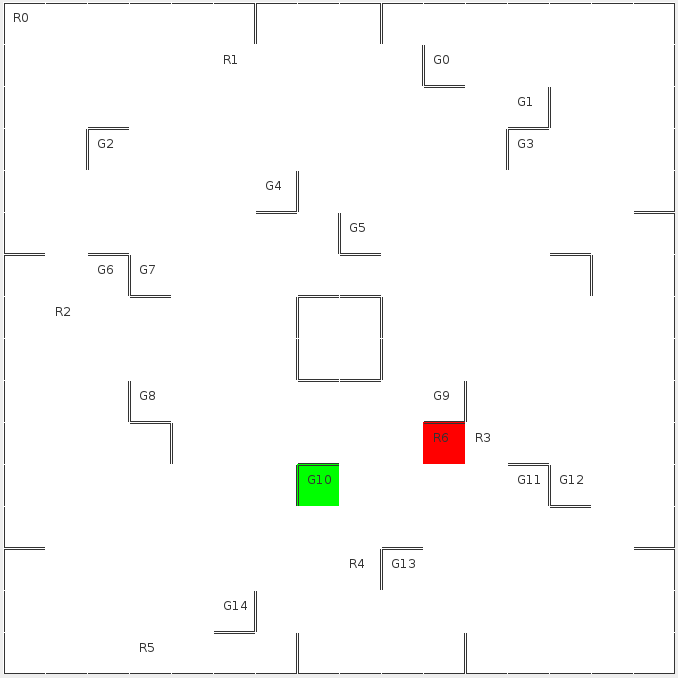
\includegraphics[height=2.6cm, width=10cm]{images/visuBoard.png}}
\institute{Université de Caen Normandie}

\begin{document}

\begin{frame}[plain]
%	\includegraphics[scale= 0.2]{LogoUNICAENv.png}
	\titlepage 
\end{frame}

\begin{frame}[plain]
\Large{Table des matières :}
	\tableofcontents[hideallsubsections]
\end{frame}

%\insertpagenumber %Pour avoir un numéro de page
%%%%%%%%%%%%%%%%%%%%%%%%%%%%%%%%%%%INFOS%%%%%%%%%%%%%%%%%%%%%%%%%%%%%%%%%%%%%%%%%%%%%%%%
%
%Grille d’évaluation de l’oral (5 points) :
%	• Diaporama non surchargé mais présentant des informations pertinentes (1 point)
%	• La présentation orale et la démonstration se sont faites dans les temps (1 point)
%	• Explication claire du projet et des points principaux (1 point)
%	• Démonstration de l’application correctement préparée (1 point)
%	• Réponses correctes aux questions du jury (1 point)
%
%1. Préparez un diaporama  2. Pas de diapositives trop chargées, pas de diapositives %vides    3. Numérotez les diapositives    4. Répartissez-vous équitablement la parole    %5. Ne lisez pas votre texte    6. Tout ce qui est dans le rapport n’a pas vocation à %être à l’oral    7. Mettez en valeur votre réalisation    8. Assurez-vous de la %lisibilité des diagrammes et images    9. Préparez votre démonstration à l’avance %%%%%%(faites une vidéo)
%%%%%%%%%%%%%%%%%%%%%%%%%%%%%%%%%%%INFOS%%%%%%%%%%%%%%%%%%%%%%%%%%%%%%%%%%%%%%%%%%%%%%%%


%MAX 25 diapos !


%--------------Partie 1--------------%
%\begin{frame}[plain]
%\tableofcontents
%\end{frame}


\section{Partie 1 - Introduction, choix du sujet}
	\subsection{Partie 1.1 - Introduction}
\begin{frame}[plain]
\frametitle{Partie 1 : Introduction, choix du sujet}
\framesubtitle{Qu'est-ce que le jeu de Ricochet Robot ?}
C'est un jeu de plateau où un robot doit atteindre une cible en faisant le moins de mouvements possibles.
\begin{figure}
	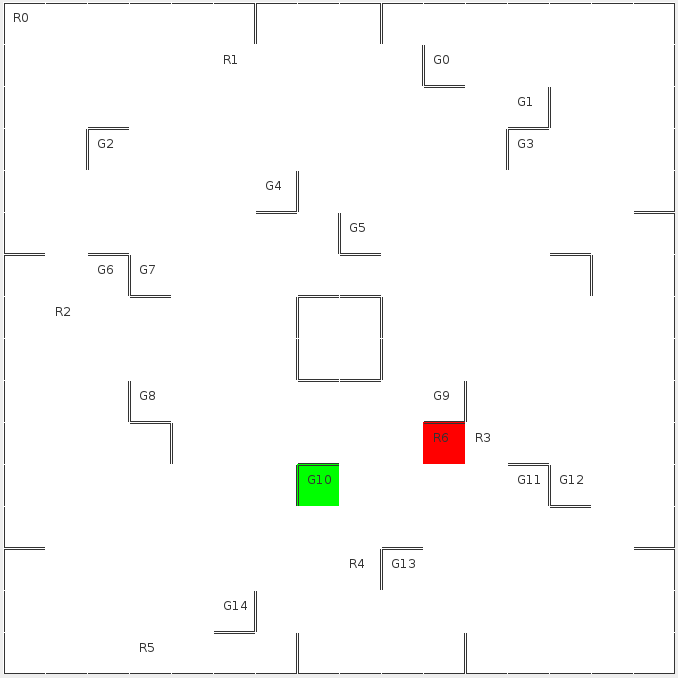
\includegraphics[width=10cm]{images/visuBoard.png}
	\caption{Jeu de Ricochet Robot}
\end{figure}
\end{frame}

	\subsection{Partie 1.2 - Choix du sujet}
\begin{frame}[plain]
\frametitle{Partie 1 - Introduction, choix du sujet}
\framesubtitle{1.2 - Choix du sujet}
\begin{alertblock}{Pourquoi avoir choisi ce sujet ?}
	\begin{itemize}
		\item Concept du jeu intéressant
		\item Implémentation d'un algorithme A*
	\end{itemize}
\end{alertblock}
\bigbreak
\begin{exampleblock}{Constitution de l'équipe}
Par affinité 
\end{exampleblock}
\end{frame}

%--------------Partie 2--------------%
\section{Partie 2 - Le moteur de jeu}
	\subsection{Partie 2.1 - Le plateau de jeu}
\begin{frame}[plain]
\begin{alertblock}{La classe Board}
	\begin{itemize}
		\item Plateau de 16*16 : il contient 256 Cases
		\item Dispose des positions des Robots et des Cibles
	\end{itemize}
\end{alertblock}

\begin{exampleblock}{Construction du plateau}
Utilisation et explication de la méthode addWall \& loadBoard
\end{exampleblock}
%classe Board. Expliquer les cases, 
%comment il est construit. addWall
\end{frame}


	\subsection{Partie 2.2 - Les robots et les cibles(Goal)}
\begin{frame}[plain]
\begin{exampleblock}{La classe Robot}
	\begin{itemize}
		\item Dispose d'un identifiant et d'une Position.
		\item Est placé aléatoirement sur la plateau grâce à la méthode loadBoard.
		\item Un Robot est choisi aléatoirement pour devenir le robot principal : takeRobot.
	\end{itemize}
\end{exampleblock}
\begin{exampleblock}{La classe Goal}
	\begin{itemize}
		\item Dispose d'un identifiant et d'une Position.
		\item Est placé aléatoirement sur la plateau grâce à la méthode loadBoard.
		\item Une Cible est choisi aléatoirement pour devenir la cible principale : takeGoal.
	\end{itemize}
\end{exampleblock}
%Qu'est-ce qu'un robot ? %et leur mise en place sur le plateau
%Qu'est-ce qu'une cible ? %et leur mise en place sur le plateau
\end{frame}


	\subsection{Partie 2.3 - Les déplacements des robots}
\begin{frame}[plain]
\begin{alertblock}{Fonctionnement d'un déplacement d'un robot}
	\begin{itemize}
		\item Uniquement en ligne droite suivant les quatre directions cardinales.
		\item Ne peut plus se déplacer lorsqu'il rencontre un mur ou un autre robot.
	\end{itemize}
\end{alertblock}
\begin{alertblock}{Méthodes de déplacement d'un robot}
	\begin{itemize}
		\item Les trois méthodes de déplacement et leurs usages : move moveRobot \& moveRobotToPosition.
		\item Les deux méthodes getAllMoves et leur utilisation.
	\end{itemize}
\end{alertblock}
%Expliquer le déplacement d'un robot
%Expliquer la méthode qui le permet
\end{frame}


	\subsection{Partie 2.4 - Autres méthodes nécessaires 1}
\begin{frame}[plain]
\begin{exampleblock}{La classe Goal}
	\begin{itemize}
		\item Dispose d'un identifiant et d'une Position.
		\item Est placé aléatoirement sur la plateau grâce à la méthode loadBoard.
		\item Une Cible est choisi aléatoirement pour devenir la cible principale : takeGoal.
	\end{itemize}
\end{exampleblock}
\begin{exampleblock}{L'aléatoire dans le jeu}
Utilisation d'un Random stocké dans la classe Board.
Utilisation dans plusieurs méthodes tels que : takeRobot, takeGoal.
\end{exampleblock}


	\subsection{Partie 2.5 - Autres méthodes nécessaires 2}
\begin{exampleblock}{Savoir s'il y a un Robot sur une case précise}
isRobot et les isRobotN/isRobotW/isRobotS/isRobotW qui permettent de savoir s'il y a Robot sur une case adjacente.
IsMainRobot qui permet de savoir si le robot principal est présent à la position donnée en paramètre.
\end{exampleblock}
\begin{exampleblock}{La Case est une Cible ou la cible principale ?}
Description de la méthode isGoal et isMainGoal
\end{exampleblock}

\begin{exampleblock}{La fin du jeu}
Précision de la méthode isFinished
\end{exampleblock}

%L'aléatoire dans le jeu(au début quand on )
%robot présent sur une case? isRobot \& isMainRobot
%Est-ce bien l'objectif ? isGoal \& isMainGoal
%La fin du jeu. isFinished
\end{frame}


%--------------Partie 3--------------%
\section{Partie 3 : algorithme A* et BFS}
	\subsection{Partie 3.1 - A*}
		\subsubsection{Partie 3.1.1 - Fonctionnement de A*}
\begin{frame}[plain]
\begin{exampleblock}{Présentation de l'algorithme A*}
	\begin{itemize}
		\item Est un algorithme qui permet de trouver rapidement une solution.
		\item Calcul d'un coût heuristique pour déterminer le prochain meilleur mouvement.
	\end{itemize}
\end{exampleblock}


\end{frame}
		\subsubsection{Partie 3.1.2 - Implémentation de A*}
\begin{frame}[plain]
\begin{alertblock}{Explication du A*}
	\begin{itemize}
		\item La liste fermée et ouverte.
		\item La méthode de recherche d'un meilleur noeud (faible coût heuristique.
	\end{itemize}
\end{alertblock}
%Explications sur le A*
\end{frame}
%ajouter autant de frame qu'il faut

	\subsection{Partie 3.2 - Le Breadth First Search ou BFS}
		\subsubsection{Partie 3.2.1 - Fonctionnement du BFS}
\begin{frame}[plain]
\begin{exampleblock}{Présentation de l'algorithme BFS}
	\begin{itemize}
		\item Trouve toujours la meilleure solution car il parcourt en largeur les noeuds.
		\item Utilise énormément d'espace.
	\end{itemize}
\end{exampleblock}
%Présentation de l'algorithme BFS
\end{frame}

		\subsubsection{Partie 3.2.2 - Implémentation du BFS}
\begin{frame}[plain]
\begin{alertblock}{Explication du BFS}
	\begin{itemize}
		\item Ajout du noeud source dans un ArrayList de Noeuds.
		\item Ajout de tous les noeuds enfants du noeud parent
		\item Si un des noeuds enfants permet de résoudre la problème alors le jeu s'arrête et la solution est retournée
		\item Si la profondeur donnée arrive à zéro, le jeu nous indique qu'il ne trouve pas de solution.
	\end{itemize}
\end{alertblock}
%Explications sur le BFS
\end{frame}
%ajouter autant de frame qu'il faut


	\subsection{Partie 3 : Comparaison des deux algorithmes}
\begin{frame}[plain]
\begin{exampleblock}{Présentation de l'algorithme BFS}
	\begin{itemize}
		\item A* : Algorithme rapide mais heuristique complexe.
		\item BFS : Algorithme qui garanti la solution optimale au détriment de la mémoire.
	\end{itemize}
\end{exampleblock}


\end{frame}

%--------------Partie 4--------------%
\section{Partie 4 : implémentation graphique et structure MVC}
\begin{frame}[plain]
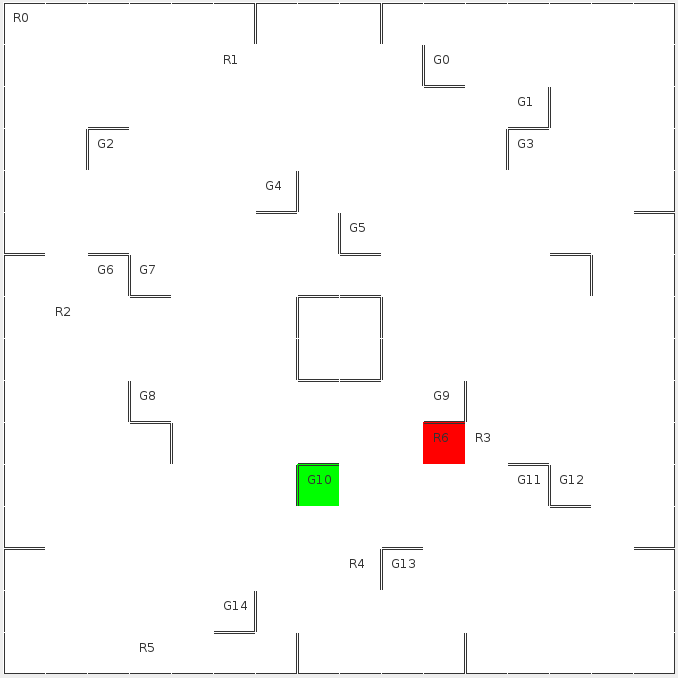
\includegraphics[height=2.2cm, width=8cm]{images/visuBoard.png}
\end{frame}


	\subsection{Partie 4.1 - Notre interface graphique et ce qu'elle contient}
\begin{frame}[plain]
Utilisation d'un JPanel qui contient : 
	\begin{itemize}
		\item Le Board
			\begin{itemize}
				\item Visualisation du plateau de jeu et jouable à travers les flèches directionnelles du clavier.
			\end{itemize}
		\item La VueMenu 
			\begin{itemize}
				\item Contenant différents boutons permettant d'enregistrer une partie, de changer de la plateau, de charger une partie, d'utiliser le A* et le BFS.
			\end{itemize}
	\end{itemize}

%Présentation de l'interface et du JPanel qui contient le Board et la VueMenu.
%Explication des boutons<------- OUI ou NON ?
\end{frame}
	%Par sûr
	
	
	\subsection{Partie 4.2 - Fonctionnement de notre structure MVC}
\begin{frame}[plain]
\begin{itemize}
	\item Un modèle qui écoute sur le clavier ou les clics que les boutons
	\item Un modèle qui met à jour la visualisation du plateau
\end{itemize}
\end{frame}

%--------------Partie 5--------------%
\section{Partie 5 : conclusion}
	\subsection{Expérimentations}
\begin{frame}[plain]
Expérimentations en terme de temps  -->Voir Yoann si je me souviens bien
Expérimentations en terme de coût (nombre de noeuds parcourus) -->Voir yoann pareil
\end{frame}
	\subsection{Partie 5.1 - Améliorations possibles}
\begin{frame}[plain]
Liste des améliorations possibles :
\begin{enumerate}
	\item Un timer.
	\item Scores multijoueur.
	\item Editeur de plateau graphique.
	\item Amélioration des algorithmes de recherche.
	\item Amélioration de l'interface graphique (sélection par clic des Robots et Cibles).
\end{enumerate}

\end{frame}

	\subsection{Pour conclure}\vspace*{\fill}
\centering Nous vous remercions pour votre écoute
\vspace*{\fill}
\hspace{0pt}
\vfill
Centered text.
\vfill
\hspace{0pt}
%\medbreak
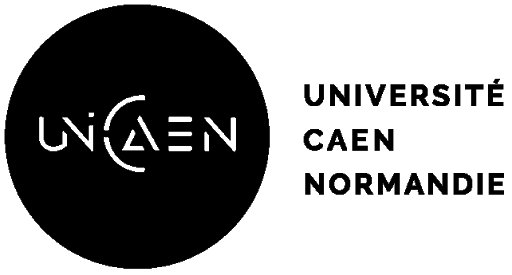
\includegraphics[scale=0.4]{images/unicaen.png}
\end{document}
